\documentclass{beamer}
\usepackage[utf8]{inputenc}
\usetheme{default}
\usecolortheme{dove}
\usepackage{textpos}
\usepackage{grid-system}
\usepackage{hyperref}
\usepackage[official]{eurosym}


\newcommand{\centeredimage}[2][ ]{
        \begin{center}
            \includegraphics[width=\textwidth,height=0.6\textheight,keepaspectratio]{#2} $\;$

            \tiny{#1}
        \end{center}
}


% po4a: environment frame
% po4a: environment Row
% po4a: environment Cell


\title{Freifunk Darmstadt}
\author{
\includegraphics[width=4cm]{../global/images/freifunk_logo}}
%\institute[Inst.]{Freifunk Darmstadt}
\date{29. Januar 2014}

\begin{document}

\begin{frame}
\maketitle
\end{frame}

\addtobeamertemplate{frametitle}{}{%
\begin{textblock*}{100mm}(0.93\textwidth,-0.5cm)

\includegraphics[height=1cm]{../global/images/freifunk_logo}
\end{textblock*}}

\begin{frame}{Themen}
\tableofcontents
\end{frame}

\section{Was ist Freifunk?}
\begin{frame}{Was ist Freifunk?}
\begin{itemize}
	\item Teil einer weltweiten Bewegung zur Etablierung von offenen und freiem Netzzugang
	\item neben der Bereitstellung eines Internetzugangs auch Plattform für lokale Dienste
	\item dezentral und gemeinschaftlich von Bürgern, Vereinen, Unternehmern und Institutionen betrieben
	\item robuste Netzwerktopologie durch Verwendung von Mesh-Netzwerken und dezentralen Routingalgorithmen
	\item Freifunk Darmstadt: Initiative des Chaos Darmstadt e.V.
\end{itemize}
\end{frame}


\begin{frame}{Was ist Freifunk?}
\framesubtitle{Freifunk in Deutschland}
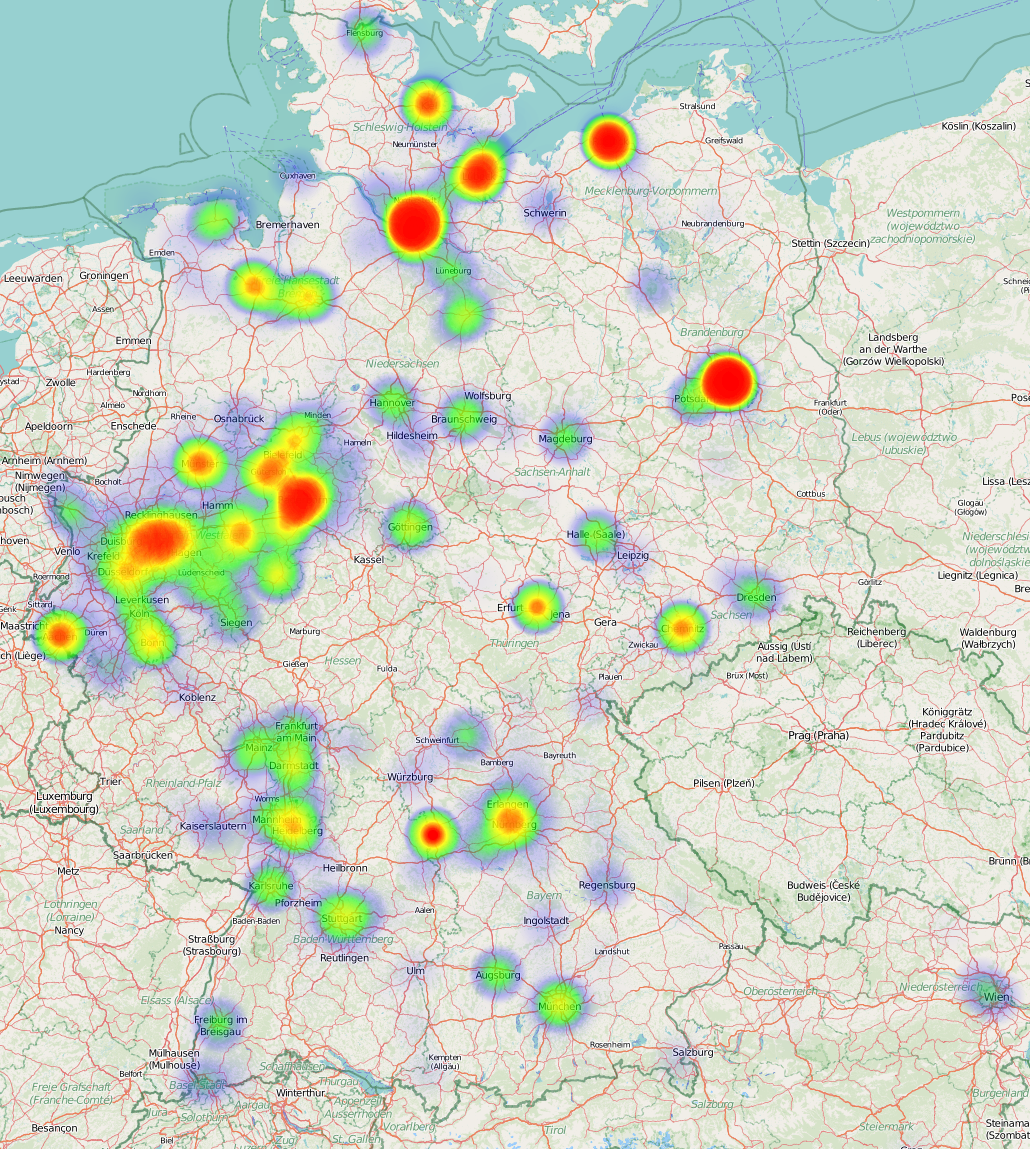
\includegraphics[height=0.6\textheight]{images/heatmap_germany} \hfill
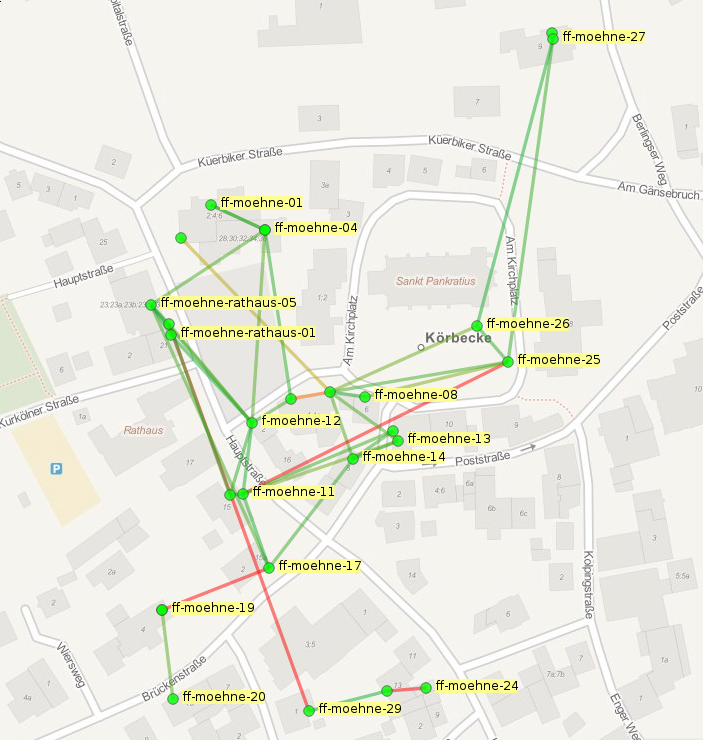
\includegraphics[height=0.6\textheight]{images/ffmap_moehne}
\end{frame}


\section{Freifunk Darmstadt}
\begin{frame}{Freifunk Darmstadt}
\framesubtitle{Knotenkarte}
\centeredimage[aktuell $\sim$ 80 Knoten in Betrieb]{images/ffmap_darmstadt}
\end{frame}

\begin{frame}{Freifunk Darmstadt}
\framesubtitle{Knotenkarte Darmstadt (City)}
\centeredimage{images/ffmap_darmstadt_city}
\end{frame}

\begin{frame}{Freifunk Darmstadt}
\framesubtitle{Knotenkarte Darmstadt (K6)}
\centeredimage{images/ffmap_darmstadt_k6}
\end{frame}

\begin{frame}{Freifunk Darmstadt}
\framesubtitle{Aufgabenbereich}
\begin{itemize}
\item Regelmäßige Informationsveranstaltungen und Workshops
\item Support bei unseren Treffen oder Online
\item Öffentlichkeitsarbeit
\item Core Team: Betrieb des Gateway-Netzes sowie der zum Betrieb notwendigen Dienste
\end{itemize}
\end{frame}


\section{Architektur}
\begin{frame}{Architektur}
\framesubtitle{Freifunk-Knoten}
\begin{itemize}
	\item Anlieger stellen Standorte zur Verfügung und betreiben eigene Freifunk-Knoten
	\item dienen als Access-Points für Endgeräte
	\begin{itemize}
		\item handelsübliche Hardware
		\item Gluon als Firmware-Framework
		\begin{itemize}
			\item Entwicklung durch deutschlandweite Community
			\item basierend auf OpenWrt $\rightarrow$ breite Hardwareunterstützung
			\item angepasste Images für verschiedene Hardwaremodelle \newline $\rightarrow$ vom Core Team erzeugt und bereitgestellt
		\end{itemize}
		\item integrierter Updatemechanismus
		\begin{itemize}
			\item Integrität und Authentizität der Updates durch kryptographische Signaturen
			\item 4-Augen-Prinzip
			\item Ausrollen binnen 24 Stunden, bei SSH-Zugang auf Knoten sogar unmittelbar auslösbar
		\end{itemize}
	\end{itemize}
\end{itemize}
\end{frame}


\begin{frame}{Architektur}
\framesubtitle{Netzaufbau}
\centeredimage{images/network_layout}
\end{frame}

\begin{frame}{Architektur}
\framesubtitle{Netzaufbau}
\begin{itemize}
	\item Knoten
	\begin{itemize}
		\item verbinden sich zum Freifunk-Netz\newline
		$\rightarrow$ über VPN oder Mesh mit sichtbaren benachbarten Knoten
		\item stellen WLAN für Clients zur Verfügung
	\end{itemize}
	\item Gateways
	\begin{itemize}
		\item dienen als Backbone zur Anbindung der Knoten
		\item stellen Basisdienste (DHCP, RA, DNS, NTP) zur Verfügung
		\item routen Traffic ins Internet (Uplink, meist über VPN-Tunnel von Drittanbietern)
	\end{itemize}
	\item zusätzliche Dienste
	\begin{itemize}
		\item Update-Server
		\item Sammlung von Metriken
		\item Monitoring
		\item \ldots
	\end{itemize}
\end{itemize}
\end{frame}

\begin{frame}{Architektur}
\framesubtitle{Ausfallsicherheit}
\vfill
\begin{itemize}
	\item mehrere Gateways zur Verbindung ins Freifunk-Netz (neben Mesh-Funktionalität)
	\item redundante Internetversorgung durch die Uplink-Gateways
	\item kontinuierliches Monitoring aller kritischen Systeme
\end{itemize}
\begin{center}
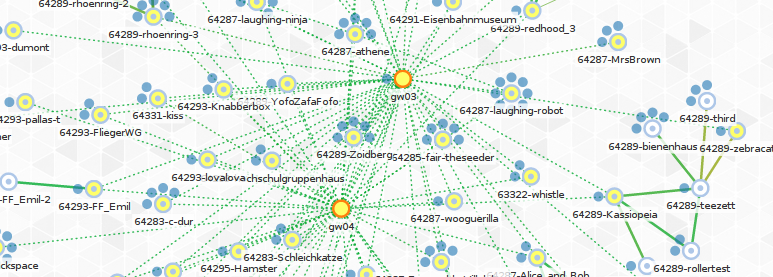
\includegraphics[width=\textwidth]{images/ffmap_graph}
\end{center}
\vfill
\small{Zeit bis zum automatischen Failover bei Ausfall eines Uplinks: max. 60s}
\vfill
\end{frame}



\section{Hardware}
\begin{frame}{Verwendete Hardware}
Handelsübliche Modelle im 2.4GHz- und 5GHz-Band
\vfill
Für den Heimbedarf oder kleinere öffentliche Bereiche:
\begin{itemize}
\item bis zu 15-25 Clients pro Gerät
\item 30-70\euro{}
\end{itemize}
\vfill

Größere Inneninstallationen:
\begin{itemize}
\item bis zu 200 Clients pro Gerät
\item 100-250\euro{}
\end{itemize}
\vfill

Größerer Außeneinsatz:
\begin{itemize}
\item bis zu 200 Clients pro Gerät
\item Kosten abhängig von verwendeten Frequenzbändern, Bandbreite und Antennentyp, 100-600\euro{}
\end{itemize}
\vfill
\end{frame}




\section{Standorte}
\begin{frame}{Standorte}
Freifunk bietet für viele Anwendungsfelder eine kosteneffiziente Möglichkeit, freien Netzzugang anzubieten:\newline
\begin{itemize}
	\item öffentliche Plätze, Staatstheater, Haltestellen, Krankenhäuser
	\item Hotels, Gaststätten, öffentliche Einrichtungen
	\item Parks (z.B. Herrengarten, Prinz-Emil-Garten)
	\item private Wohnungen, Studentenwohnheime
	\item hochgelegene Plätze für Richtfunk (z.B. Langer Ludwig, Kirchtürme, Hochzeitsturm, h$\_$da Hochhaus)
\end{itemize}
\end{frame}



\section{Konzept: Luisenplatz}
\begin{frame}{Konzept: Luisenplatz}
\framesubtitle{Vogelperspektive}
\centeredimage{images/plan_luisenplatz1.jpg}
\end{frame}

\begin{frame}{Konzept: Luisenplatz}
\framesubtitle{Hardwarevorschlag}
Annahme: Montage der Freifunk-Knoten auf den Anzeigesäulen der HEAG mobilo


\begin{minipage}{0.4\textwidth} 
\begin{itemize}
	\item UniFi AP AC Outdoor
	\item Abmessungen: 200x204x27mm
	\item Gewicht: 600g
	\item Stromverbrauch: maximal 22W
	\item Dualband, 802.11ac
	\item Reichweite: 183m
	\item 3x3 MIMO
\end{itemize}
% \caption{Der Text}
% \label{Text}
\end{minipage}
% Auffüllen des Zwischenraums
\hfill
% minipage mit Grafik
\begin{minipage}{0.4\textwidth}
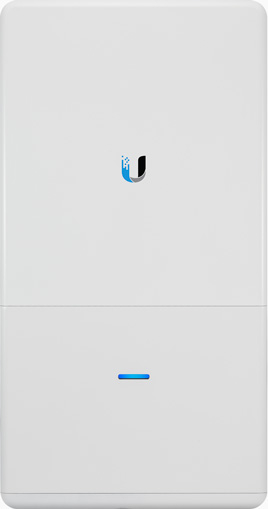
\includegraphics[width=0.8\textwidth]{images/unifi-ap-ac-outdoor.jpg}
\end{minipage}



\end{frame}
\begin{frame}{Konzept: Luisenplatz}
\framesubtitle{Positionierung der Knoten}

\centeredimage{images/plan_luisenplatz2.jpg}
\end{frame}

\begin{frame}{Konzept: Luisenplatz}
\framesubtitle{prognostizierte Ausleuchtung}
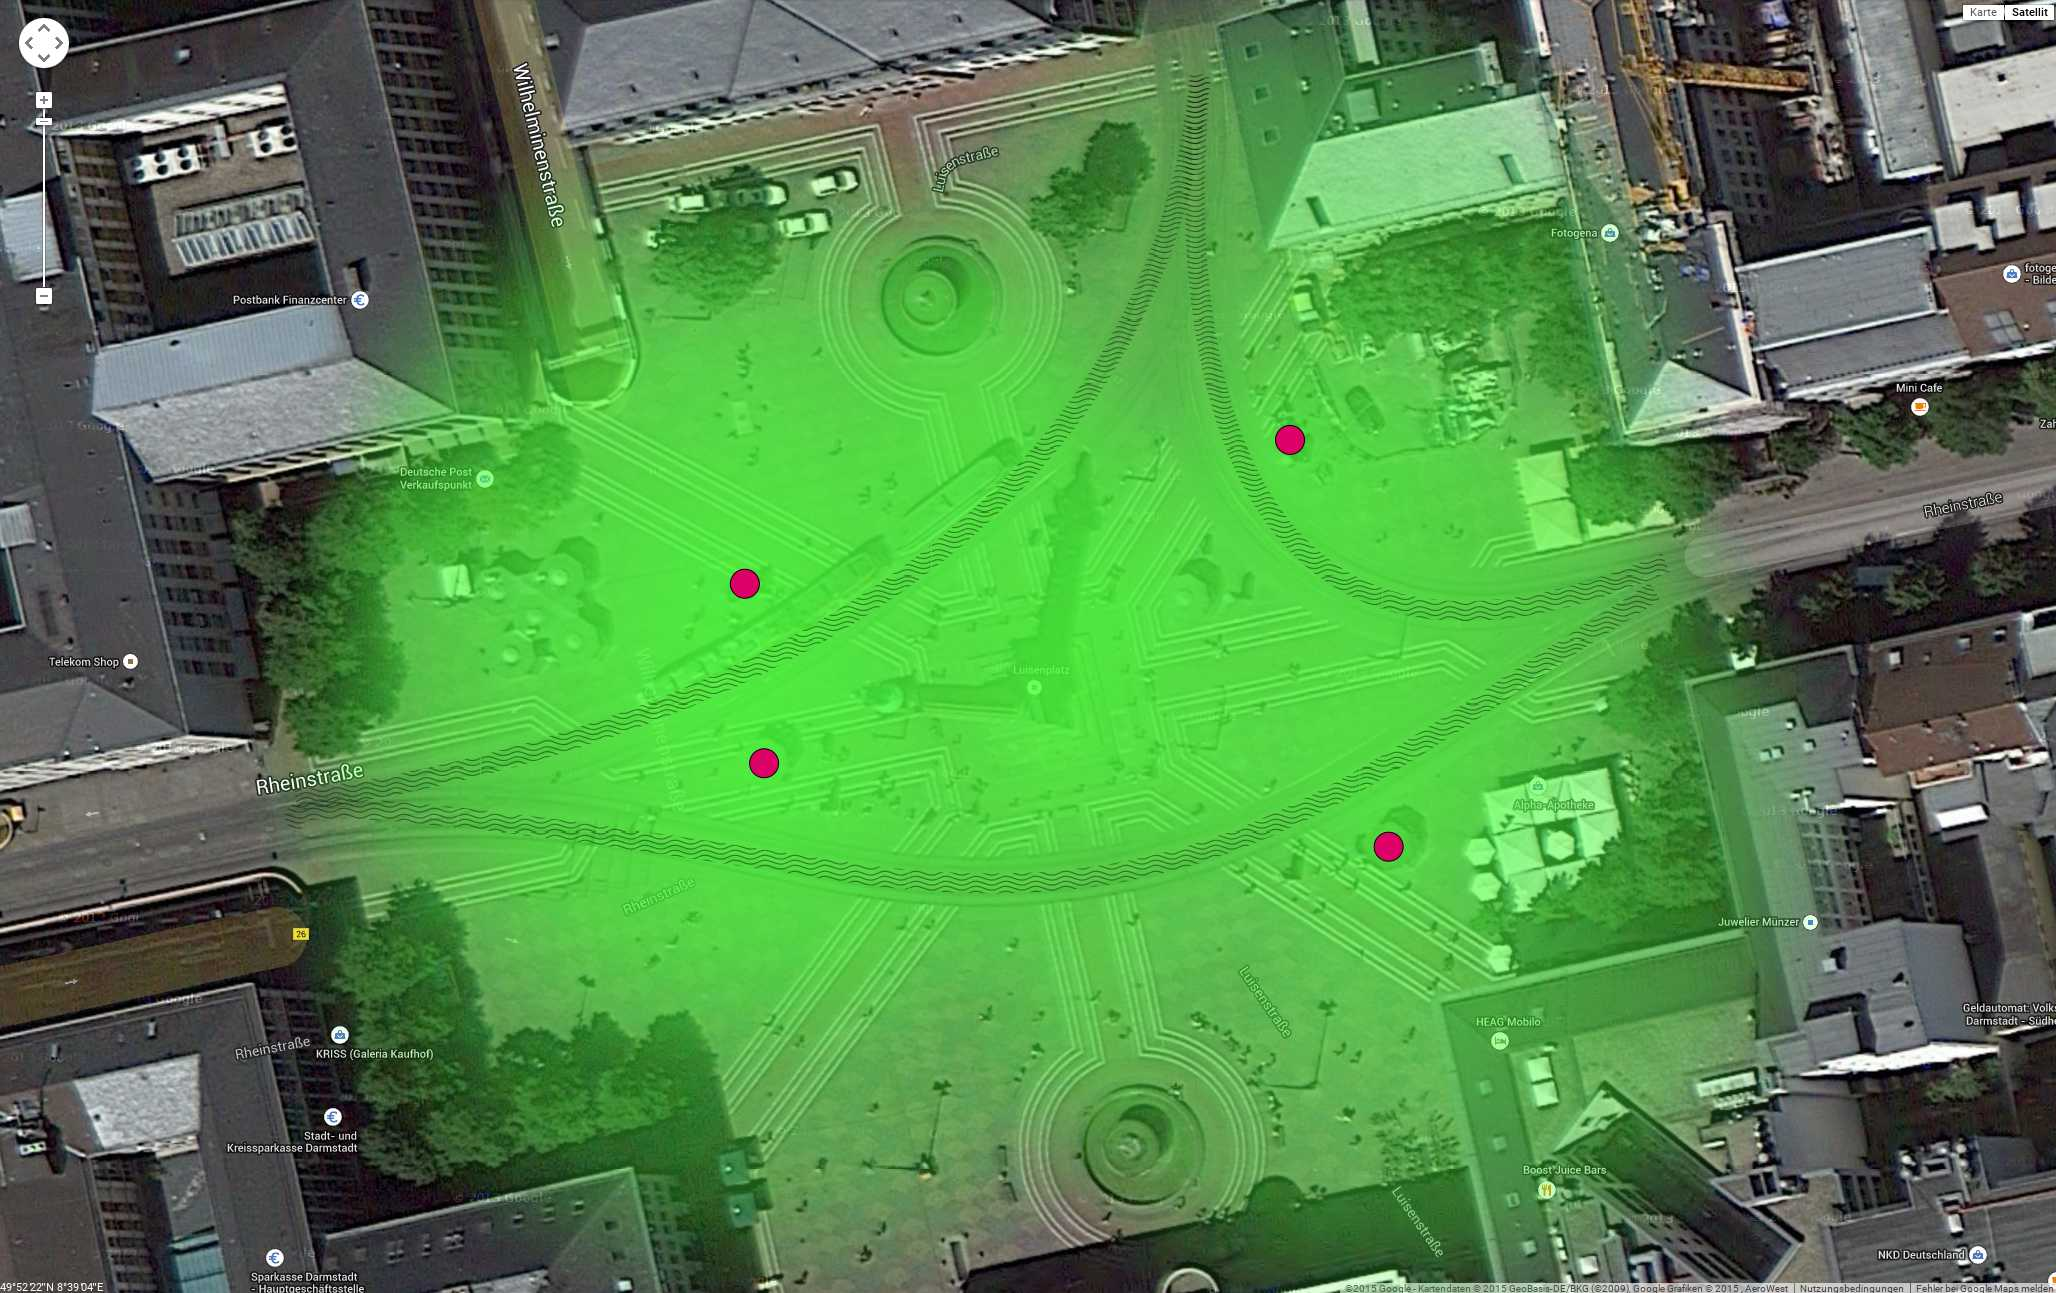
\includegraphics[height=0.75\textheight]{images/plan_luisenplatz3.jpg}
\end{frame}

\begin{frame}{Konzept: Luisenplatz}
\framesubtitle{Anforderungen an die Stadt}
\vfill
\begin{center}
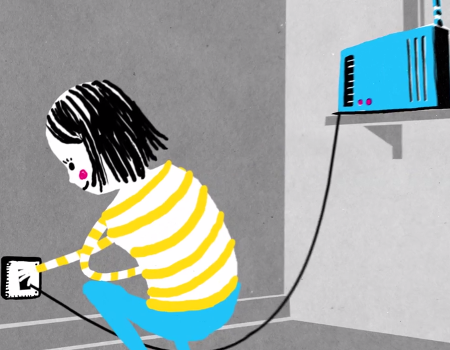
\includegraphics[height=0.4\textheight]{../global/images/freifunk_setup}$\;$
\vfill
\end{center}
\begin{itemize}
\item Bereitstellung von Standorten/Montageflächen
\item Bereitstellung von Strom und Internetanbindung (alternativ Anbindung über Richtfunk)
\item Erwerb oder Sponsoring der notwendigen Hardware
\item Durchführung fachgerechter Montagearbeiten (standortabhängig)
\end{itemize}
\vfill
\end{frame}

\begin{frame}{Konzept: Luisenplatz}
\framesubtitle{Grobkalkulation}
Anschaffungskosten:
\begin{itemize}
	\item 4x UniFi AP AC Outdoor (390\euro{} inkl. MwSt.) = 1560\euro{}
	\item Controller-Hardware ($\sim$ 1000\euro{})
	\item notwendige Montagearbeiten und Abnahme
\end{itemize}
\vfill
Laufende Kosten:
\begin{itemize}
	\item Stromkosten Router (Herstellerangabe Maximalverbrauch 22W):\newline
	192kWh/Jahr je Gerät $\rightarrow$ max. 768kWh/Jahr
	\item Stromkosten Controller-Hardware \newline
	($\sim$150W) $\rightarrow$ 1314 kWh/Jahr
	\item Beitrag zur Finanzierung der Backbone-Infrastruktur: \newline
	2000 \euro{} / Jahr
\end{itemize}
\end{frame}


\section{Kooperationen in anderen Städten}
\begin{frame}{Kooperationen in anderen Städten}
\begin{itemize}
\item Berlin und Lübeck, Weimar: Zugang zu den Dächern öffentlicher Gebäude zum Aufbau eines Richtfunknetzes \newline $\rightarrow$ unabhängige Infrastruktur in Bürgerhand
\item Medienanstalt Berlin-Brandenburg: Förderung im Rahmen der WLAN-Initiative PUBLIC WIFI, Broschüre
\item Arnsberg: Förderung durch Verkehrsverein, Sponsor: regionale Sparkasse
\item Rothenburg: Kontakt zu lokalen Geschäften, Bereitstellung vorkonfigurierter Router durch Rothenburger Stadtmarketing
\end{itemize}
\end{frame}


\section{Weitere mögliche Schritte}
\begin{frame}{Weitere mögliche Schritte in Darmstadt}
\begin{itemize}
\item Bereitstellen von lokaler Dienste im Freifunk-Netz (Bürgerinformationen, Aktuelles aus Darmstadt und Umgebung, \ldots)
\item Versorgung weiterer Standorte mit freiem Netzzugang
\begin{itemize}
	\item öffentliche Plätze und Gebäude
	\item Parkanlagen
	\item Einkaufspassagen (Darmstädter Citymarketing)
\end{itemize}
\item Aufbauen von Richtfunkstrecken über größere Distanz (von höheren Standorten aus)
\begin{itemize}
	\item Langer Lui
	\item Hochzeitsturm
\end{itemize}
\end{itemize}
\vfill
\end{frame}

\begin{frame}
\begin{center}
\Huge Fragen?
\end{center}
\end{frame}


\begin{frame}
\begin{center}
\Huge Vielen Dank für Ihre Aufmerksamkeit!
\end{center}
\end{frame}

\begin{frame}{Quellen/Bildnachweise}
\begin{itemize}
	\item Freifunk-Logo: CC BY-SA 3.0 \href{http://freifunk.net}{freifunk.net}
	\item Kartendaten: © \href{http://openstreetmap.org}{OpenStreetMap} contributors
	\item Luftbildaufnahme Luisenplatz: © 2015 Aero West, Google, Kartebdaten © 2015 GeoBasis-DE/BKG(© 2009), Google
	\item UniFi AP AC Outdoor:  \href{ubnt.com}{ubnt.com}
	\item Bild "Inbetriebnahme Freifunk-Router": CC BY-SA 3.0 \href{http://freifunk.net}{freifunk.net}
\end{itemize}
\end{frame}

\begin{frame}{Weitere Informationen}
\begin{itemize}
	\item \href{http://freifunk-darmstadt.de}{freifunk-darmstadt.de}
	\item \href{http://map.freifunk-darmstadt.de}{map.freifunk-darmstadt.de}
	\item \href{http://gluon.readthedocs.org}{gluon.readthedocs.org}
	\item \href{http://paderborn.freifunk.net/?page_id=42}{Pico Peering Agreement}
	\item \href{http://mabb.de/files/content/document/Publikationen/Freifunk-Broschuere/freifunk_publikation_webversion.pdf}{Broschüre der Medienanstalt Berlin-Brandenburg}
\end{itemize}
\end{frame}


\end{document}
